%==========================================================================
%  Software implementation of the time-dependent Dual TRILEX scheme
%  with a full three-point vertex
%==========================================================================

\documentclass[10pt,aspectratio=169]{beamer}

% ---------- Theme ---------------------------------------------------------
\usetheme{Madrid}
\usecolortheme{seahorse}
\useinnertheme{rectangles}
\useoutertheme{infolines}
\setbeamertemplate{navigation symbols}{}

% ---------- Packages ------------------------------------------------------
\usepackage[utf8]{inputenc}
\usepackage[T1]{fontenc}
\usepackage{lmodern}
\usepackage{amsmath,amssymb,bm}
\usepackage{graphicx}
\usepackage{tikz}
\usetikzlibrary{arrows.meta,calc,decorations.pathmorphing,positioning}
\usepackage{listings}
\usepackage{xcolor}
\usepackage{hyperref}
\usepackage{booktabs}
\usepackage{qrcode}

% ---------- Math shortcuts -----------------------------------------------
\newcommand{\qv}{\mathbf{q}}
\newcommand{\kv}{\mathbf{k}}
\newcommand{\Sigmat}{\Sigma}
\newcommand{\Lam}{\Lambda}
\newcommand{\trilex}{D\nobreakdash-TRILEX}
\newcommand{\dgw}{D\nobreakdash-$GW$}
\newcommand{\realevol}{\texttt{realevol}}
\newcommand{\tddt}{\texttt{tddt}}
\newcommand{\triqs}{\textsc{triqs}}

% ---------- Listings style for code snippets -----------------------------
\definecolor{kwcol}{HTML}{0033B3}
\definecolor{strcol}{HTML}{067D17}
\definecolor{commcol}{HTML}{8C8C8C}
\lstset{
  basicstyle=\ttfamily\scriptsize,
  keywordstyle=\color{kwcol}\bfseries,
  stringstyle=\color{strcol},
  commentstyle=\color{commcol}\itshape,
  showstringspaces=false,
  breaklines=true,
  frame=single,
  framerule=0.4pt,
  rulecolor=\color{black!25},
  language=Python,
  numbers=none
}

% ---------- Title block ---------------------------------------------------
\title[Time-dependent Dual TRILEX implementation]{%
  Software implementation of the time-dependent Dual TRILEX scheme\\
  with a full three-point vertex}
\subtitle{}
\author[I.\,Krivenko et al]{\underline{Igor Krivenko}, Viktor Harkov,
        Evgeny A. Stepanov, Viktor Valmispild, Patryk Kubiczek,
        Alexander.~I.~Lichtenstein}
\date[ERC-FASTCORR 2026]{ERC FASTCORR meeting\\May 25, 2026}

% =========================================================================
\begin{document}

% --- 1. Title slide -------------------------------------------------------
\begin{frame}
  \titlepage
\end{frame}

% --- 2. Outline -----------------------------------------------------------
\begin{frame}{Outline}
  \begin{enumerate}
    \item Motivation: Real-time D-TRILEX with the full three-point vertex
    \item Short reminder of the (equilibrium) D-TRILEX construction
    \item Time-dependent D-TRILEX on the two-branch Keldysh contour
    \item A short-time propagation scheme for finite systems with $\hat H(t)$
    \item \realevol: a \triqs-based real-time impurity solver
          \emph{including} measurement\\ of the exact 3-point vertex
    \item \tddt: the Python package implementing the rest of
          the time-dependent\\ D-TRILEX scheme (calls \realevol\ to solve the reference system)
    \item Status, current bottlenecks, outlook
  \end{enumerate}
\end{frame}

% =========================================================================
\section{Motivation}
% =========================================================================

% --- 3. Why non-equilibrium with strong correlations ----------------------
\begin{frame}{Why non-equilibrium correlated electrons?}
  \begin{columns}[T,onlytextwidth]
    \begin{column}{0.58\textwidth}
      \textbf{Pump-probe experiments} now resolve dynamics on the
      femtosecond scale in correlated materials:
      \begin{itemize}
        \item light-induced superconductivity, hidden phases,
        \item ultrafast demagnetisation, photo-doping,
        \item dielectric breakdown of Mott insulators.
      \end{itemize}

      \vspace{0.5em}
      \textbf{Theoretical challenge.} Need to describe simultaneously:
      \begin{itemize}
        \item strong local correlations (Mott physics),
        \item non-local charge and spin fluctuations (collective modes),
        \item explicit time dependence $\hat H = \hat H(t)$.
      \end{itemize}
    \end{column}
    \begin{column}{0.40\textwidth}
      \begin{block}{Available methods today}
        \footnotesize
        \begin{itemize}
          \item Non-equilibrium DMFT - local self-energy only;
          \item $GW$+EDMFT - charge fluctuations, no spin;
          \item TPSC+DMFT - both, but small $U$;
          \item \dgw\ (instantaneous vertex) - recent work by N. Dasari {\it et al}.
        \end{itemize}
      \end{block}
      \footnotesize
      \emph{None} of these uses the full frequency- / time-dependent
      three-point vertex out of equilibrium.
    \end{column}
  \end{columns}
\end{frame}

% --- 4. The vertex problem ------------------------------------------------
\begin{frame}{The three-point vertex problem out of equilibrium}
  Equilibrium D-TRILEX is built around the exact three-point vertex
  $\Lambda(\nu,\omega)$ of the DMFT impurity:
  \[
    \tilde\Sigma_{k,\nu}
    \;\sim\;
    \sum_{q,\omega}\,
    \Lambda(\nu,\omega)\,
    \tilde G_{k+q,\nu+\omega}\,
    W(q,\omega)\,
    \Lambda(\nu,\omega).
  \]
  \medskip

  \textbf{Out of equilibrium}, on the two-branch Keldysh contour
  $\mathcal{C}=\mathcal{C}_+\cup\mathcal{C}_-$ with initial density
  matrix $\rho_0$:
  \begin{itemize}
    \item $\Lambda(\nu,\omega) \to \Lambda(t_1,t_2,t_3)$ — a \emph{three-time} object;
    \item Self-energy / polarization acquire \textbf{four contour-time}
          integrals;
    \item Generalized Langreth rules become combinatorially heavy
          (cf.\ Kugler et al., PRX {\bf 11}, 041006 (2021)).
  \end{itemize}

  \begin{alertblock}{The pragmatic compromise so far}
    The recent real-time \dgw\ paper (Dasari et al., PRB 111, 235129 (2025)) keeps only the
    \emph{instantaneous} ($t_1=t_2=t_3$) part of $\Lambda$ - equivalent
    to a $GW$+DMFT-like diagrammatic structure.\\
    \textbf{Goal of this work:} keep the \emph{full} time-dependent
    three-point vertex.
  \end{alertblock}
\end{frame}

% --- 5. Project goal ------------------------------------------------------
\begin{frame}{What this talk is about}
  Two pieces of software, developed within the FASTCORR project,
  that together realise the time-dependent D-TRILEX scheme with the
  \textbf{full} three-point vertex:

  \vspace{1em}
  \begin{columns}[T]
    \begin{column}{0.48\textwidth}
      \begin{block}{\realevol\ (\triqs/C++/Python)}
        \footnotesize
        Real-time impurity solver based on \triqs.\\[2pt]
        For a finite system, computes by exact propagation:
        \begin{itemize}
          \item impurity Green's function $G(t,t')$,
          \item susceptibilities $\chi(t_1,t_2)$,
          \item \textbf{exact three-point vertex}
                $\Lambda(t_1,t_2,t_3)$.
        \end{itemize}
      \end{block}
    \end{column}
    \begin{column}{0.48\textwidth}
      \begin{block}{\tddt\ (\triqs/Python)}
        \footnotesize
        Lattice solver of the time-dependent D-TRILEX equations:
        \begin{itemize}
          \item contour-time Green's functions \& bosonic
                propagators on the Keldysh contour,
          \item correlated initial state from exact diagonalization,
          \item self-energy / polarization built from
                \realevol\ vertices and dual lines,
          \item dual Dyson equation on the contour,
          \item correlators of physical electrons from the dual ones.
        \end{itemize}
      \end{block}
    \end{column}
  \end{columns}
  \vspace{0.7em}
  Both are open-source (GPLv3), \texttt{github.com/krivenko/\{triqs-realevol,tddt\}}.
\end{frame}

% =========================================================================
\section{Reminder: D-TRILEX}
% =========================================================================

\begin{frame}{D-TRILEX in one slide (equilibrium)}
  \begin{columns}[T,onlytextwidth]
    \begin{column}{0.50\textwidth}
      \small
      Start from a lattice action with local $U$ and non-local
      interaction $V_{ij}$. Introduce a DMFT-like reference and rewrite
      in dual variables.

      \medskip
      \textbf{Key ingredients} (from the impurity):
      \begin{itemize}
        \item local Green's function $g_\nu$,
        \item local susceptibility $\chi_\omega$,
        \item \textbf{exact} three-point vertex
              $\Lambda_{\nu,\omega}$ (charge \& spin).
      \end{itemize}

      \medskip
      \textbf{Diagrammatic content.} Single bosonic exchange dressed
      by $\Lambda$:
      \begin{itemize}
        \item $GW$-like diagrammatic complexity;
        \item accuracy of much heavier parquet-class methods;
        \item charge and spin on equal footing.
      \end{itemize}
    \end{column}
    \begin{column}{0.43\textwidth}
      \centering
      \begin{align*}
          \Sigmat_{\kv\nu\sigma} &= -\sum_{\qv,\omega,\varsigma}\Lambda^{\varsigma}_{\nu+\omega,-\omega}\tilde{G}^{\phantom{2}}_{\kv+\qv,\nu+\omega,\sigma'}W^{\varsigma}_{\qv\omega}\Lambda^{\varsigma}_{\nu,\omega}
          \\&= \vcenter{\hbox{\includegraphics[width=0.3\linewidth]{Sigma_d.pdf}}} \notag\\
          \tilde{\Pi}^{\varsigma}_{\qv\omega}  &= \sum_{\kv,\nu,\sigma(')} \Lambda^{\varsigma}_{\nu+\omega,-\omega}\tilde{G}^{\phantom{2}}_{\kv+\qv,\nu+\omega,\sigma}\tilde{G}^{\phantom{2}}_{\kv\nu\sigma'}\Lambda^{\varsigma}_{\nu,\omega}
          \\&= \vcenter{\hbox{\includegraphics[width=0.3\linewidth]{Pi_d.pdf}}}
      \end{align*}

      \vspace{0.8em}
      \footnotesize
      Stepanov \emph{et al.}, PRB 100, 205115 (2019);\\
      Harkov \emph{et al.}, PRB 103, 245123 (2021);\\
      Vandelli \emph{et al.}, SciPost Phys. 13, 036 (2022).
    \end{column}
  \end{columns}
\end{frame}

% --- 7. "Lighter" instantaneous-vertex version --------------------------
\begin{frame}{The ``lighter'' real-time \dgw\ (Dasari et al., PRB 111, 235129 (2025))}
  \small
  Recently, a non-equilibrium variant was implemented by Dasari, Strand,
  Eckstein, Lichtenstein, Stepanov:
  \begin{itemize}
    \item L-shaped Keldysh contour, two-time
          $\tilde\Sigma(t,t')$ and $\tilde\Pi(t,t')$;
    \item three-point vertex \emph{approximated by its
          instantaneous component}
          $\Lambda(t_1,t_2,t_3)\approx
           \lambda\,\delta_\mathcal{C}(t_1,t_2)\delta_\mathcal{C}(t_2,t_3)$;
    \item self-energy reduces to a $GW$+DMFT-like form, plus the
          spin channel.
  \end{itemize}

  \begin{alertblock}{What is lost}
    Frequency / time dependence of $\Lambda$ encodes \emph{retardation}
    of the coupling between fermions and collective modes.
  \end{alertblock}

  The present work aims to remove this approximation by
  \begin{enumerate}
    \item measuring $\Lambda(t_1,t_2,t_3)$ directly in real time
          (the \realevol\ part),
    \item folding it into the lattice equations on the Keldysh contour
          (the \tddt\ part).
  \end{enumerate}
\end{frame}

% =========================================================================
\section{Time-dependent D-TRILEX with the full vertex}
% =========================================================================

\begin{frame}{Time-dependent D-TRILEX: structure of equations}
  \small
  On the Keldysh contour $\mathcal{C}$ we keep the same diagrammatic
  topology as in equilibrium, but every line/vertex is a contour-time
  object.

  \medskip
  \begin{block}{Non-local self-energy}
    \[
    \tilde \Sigmat_{\bm{k}}(t,t')
    = \mathrm{i}\!\sum_{\bm{q}}\!\!\iiiint_\mathcal{C}\!\!
    \mathrm{d}\bar t_1\,\mathrm{d}\bar t_2\,
    \mathrm{d}\bar t_3\,\mathrm{d}\bar t_4\;
    \Lam(t,\bar t_1,\bar t_2)\,
    \tilde G_{\bm{k}+\bm{q}}(\bar t_1,\bar t_3)\,
    W_{\bm{q}}(\bar t_2,\bar t_4)\,
    \Lam(\bar t_3,t',\bar t_4)
    \]
  \end{block}
  \begin{block}{Polarisation operator}
    \[
    \tilde\Pi_{\bm{q}}(t,t')
    = -\mathrm{i}\!\sum_{\bm{k}}\!\!\iiiint_\mathcal{C}\!\!
    \mathrm{d}\bar t_1\,\mathrm{d}\bar t_2\,
    \mathrm{d}\bar t_3\,\mathrm{d}\bar t_4\;
    \Lam(\bar t_1,\bar t_2,t)\,
    \tilde G_{\bm{k}}(\bar t_1,\bar t_3)\,
    \tilde G_{\bm{k}+\bm{q}}(\bar t_4,\bar t_2)\,
    \Lam(\bar t_3,\bar t_4,t')
    \]
  \end{block}
  \vspace{-0.3em}
  Four contour-time integrations per Dyson iteration.\\
  Memory cost (per channel): $\mathcal{O}(N_t^3)$ for $\Lambda$,
  $\mathcal{O}(N_t^2)$ for $\tilde G$, $W$.
\end{frame}

% --- 9. Computational challenges -----------------------------------------
\begin{frame}{Computational challenges}
  \begin{itemize}
    \item \textbf{Three-time vertex} $\Lambda(t_1,t_2,t_3)$ on the
          Keldysh contour: $8$ components per $(t_1,t_2,t_3)$ triple.
    \item \textbf{Langreth-type rules}: convolutions involving three-time
          objects on a piece-wise contour are no longer reducible to a
          handful of retarded/advanced/lesser pieces.
    \item \textbf{Initial correlations} are absorbed entirely into the
          initial density matrix $\hat\rho_0$: \realevol\ accepts an
          arbitrary $\rho_0$; \tddt\ uses $\rho_0 = e^{-\beta \hat H(0)}/Z$.
          No Matsubara branch in either code.
  \end{itemize}

  \medskip
  We attack these in two independent pieces of software, glued via \triqs\ Green's-function containers.
\end{frame}

% =========================================================================
\section{Short-time propagation}
% =========================================================================

\begin{frame}{Short-time propagation for finite systems with $\hat H(t)$}
  \footnotesize Main reference: \emph{Balzer et al, J. Phys.: Condens. Matter 24 035603 (2011)}.

  \medskip
  \textbf{Problem.} Evolve $|\psi(t)\rangle$ under an explicitly
  time-dependent Hamiltonian $\hat H(t)$ acting in a finite Hilbert space
  $\mathcal{H}$ (dim$\,\mathcal{H}\sim 10^2{-}10^6$):
  \[
    \mathrm{i}\,\partial_t |\psi(t)\rangle = \hat H(t)\,|\psi(t)\rangle,
    \qquad
    \hat U(t+\Delta t,t)=\mathcal{T}\exp\Bigl[-\mathrm{i}\!\!\int_t^{t+\Delta t}\!\!\!\hat H(s)\,\mathrm{d}s\Bigr].
  \]

  \textbf{Two competing requirements:}
  \begin{itemize}
    \item \emph{unconditional stability + unitarity}
          $\to$ exclude explicit Runge-Kutta;
    \item \emph{high order in $\Delta t$ at moderate cost}
          $\to$ exclude naïve Crank-Nicolson alone.
  \end{itemize}

  \begin{block}{Strategy adopted in \realevol}
    On each step $[t_n,t_{n+1}]$, approximate $\hat H(s)$ by a single
    representative $\hat H_n$ (midpoint sampling) and apply
    $\mathrm{e}^{-\mathrm{i}\hat H_n \Delta t}$ via a Krylov subspace
    (short iterative Lanczos) projection of $\hat H_n$.
\end{block}
\end{frame}

% --- 11. Short-time propagation: scheme ----------------------------------
\begin{frame}{Short-time propagation: scheme}
  \small
  For each step $[t_n,t_{n+1}]$, with $\Delta t = t_{n+1}-t_n$:
  \begin{enumerate}
    \item \textbf{Midpoint sample}
          $\hat H_n = \hat H\!\left(t_n + \tfrac{\Delta t}{2}\right)$.
    \item \textbf{Krylov subspace}: build
          $\mathcal{K}_m = \mathrm{span}\{|\psi_n\rangle,\,\hat H_n|\psi_n\rangle,\,\dots,
                                  \hat H_n^{m-1}|\psi_n\rangle\}$
          using Lanczos iteration.
    \item \textbf{Project}: tridiagonalize $\hat H_n$ to
          $T_m \in \mathbb{C}^{m\times m}$ ($m\sim 10\text{-}30$).
    \item \textbf{Exponentiate} $\mathrm{e}^{-\mathrm{i} T_m \Delta t}$
          exactly in the small subspace.
    \item \textbf{Lift back}:
          $|\psi_{n+1}\rangle = \hat V_m\, \mathrm{e}^{-\mathrm{i} T_m \Delta t}\,
            \hat V_m^\dagger\,|\psi_n\rangle$.
  \end{enumerate}

  \medskip
  \textbf{Properties:}
  \begin{itemize}
    \item norm-preserving up to numerical precision of the projection;
    \item time-ordering captured to leading order in $\Delta t$;
    \item cost dominated by matrix–vector products with the sparse $\hat H_n$
            ; scales as $O(\mathrm{nnz}(\hat H_n))$ - quasi-linear in $\dim\mathcal H$
            for impurity-plus-bath Hamiltonians.
  \end{itemize}
\end{frame}

% --- 12. Building Green's functions from propagated states ---------------
\begin{frame}{From propagated states to Green's functions and vertices}
    \small
    \realevol\ works on the two-branch Keldysh contour
    $\mathcal{C}_+\cup\mathcal{C}_-$, with the initial state supplied as
    an \emph{arbitrary} density matrix $\hat\rho_0$ (thermal,
    post-quench, projected onto a sector, $\dots$).

    \medskip
    Given $\hat U(t,0)$, all dynamical quantities follow as
    direct traces with $\hat\rho_0$:
    \[
    G^>_{ab}(t,t') = -\mathrm{i}\,
    \mathrm{Tr}\!\left[\hat\rho_0\;
    \hat U^\dagger(t,0)\,c_a\,\hat U(t,t')\,c_b^\dagger\,\hat U(t',0)
    \right],
    \]
    and analogously for $G^<$, $G^R$, $G^A$. No analytic continuation;
    no Matsubara branch.

    \medskip
    \textbf{Three-point vertex.} Same structure with three operator
    insertions on $\mathcal{C}$:
    \[
    \Lam_{a\bar a;cd}(t_1,t_2,t_3) \sim
    \mathrm{Tr}\!\left[\hat\rho_0\,\mathcal{T}_\mathcal{C}\,
    c_a(t_1)\,c^\dagger_{\bar a}(t_2)\,
    n_{cd}(t_3)\right]_{\text{conn}}
    \]
    \\
    Eight Keldysh components per $(t_1,t_2,t_3)$ triple on
    $\mathcal{C}_+\cup\mathcal{C}_-$.

    \medskip
    \textbf{Bottleneck:} memory $\mathcal{O}(N_t^3)\times 8$ components.
\end{frame}

% =========================================================================
\section{realevol — implementation}
% =========================================================================

\begin{frame}{\realevol\ — real-time impurity solver based on \triqs}
    \begin{tikzpicture}[remember picture, overlay]
        \node[anchor=north east, xshift=-4pt, yshift=-4pt]
        at (current page.north east) {%
            \begin{tikzpicture}
                \node[fill=white, draw=black!20, inner sep=2pt, rounded corners=1pt]
                {\qrcode[height=1.6cm]{https://github.com/krivenko/triqs-realevol}};
        \end{tikzpicture}};
    \end{tikzpicture}
    \small
    \texttt{github.com/krivenko/triqs-realevol} (Python $\ge$ 3.10, \triqs\ 3.3.x).

    \medskip
    \begin{columns}[T,onlytextwidth]
        \begin{column}{0.55\textwidth}
            \textbf{Architecture}
            \begin{itemize}
                \item C++17 core with a Python wrapping
                (\texttt{cpp2py}, \triqs\ convention);
                \item exact diagonalization of a finite system of fermions;
                \item (optional) initial thermal state $\hat{\rho_0}$ from Lanczos diagonalization: \texttt{ARPACK-NG} ($\ge 3.8.0$);
                \item time propagation via Lanczos iteration (own implementation);
                \item parallel over Hilbert-space sectors (MPI);
                \item HDF5 I/O through \triqs\ archives.
            \end{itemize}
        \end{column}
        \begin{column}{0.43\textwidth}
            \textbf{What \realevol\ computes}
            \begin{itemize}
                \item initial thermal density matrix $\hat\rho_0 = e^{-\beta \hat H(0)}/Z$;
                \item one-particle $G(t,t')$ on the two-branch Keldysh contour;
                \item generalized susceptibilities $\chi(t,t')$
                (charge, spin, pairing);
                \item \textbf{exact three-time correlators}
                $\langle O_1(t_1)\,O_2(t_2)\,O_3(t_3)\rangle$
                    - the building block of $\Lambda(t_1,t_2,t_3)$;
                \item arbitrary local observables.
            \end{itemize}
        \end{column}
    \end{columns}
\end{frame}

% --- 14. realevol: workflow ----------------------------------------------
\begin{frame}[fragile]{\realevol\ — typical workflow (Python)}
    \begin{lstlisting}
    from triqs.gf import MeshReTime
    from realevol.tinterp import TInterp as ti
    from realevol.operators_tinterp import n, c, c_dag
    from realevol.init_state import make_equilibrium_init_state
    from realevol.realevol import compute_g_g, compute_g_l, compute_chi, compute_correlator_3t

    t_mesh = MeshReTime(0, t_max, n_t)

    # Initial Hamiltonian; thermal rho_0 at temperature T
    H0 = -mu*(n('up',0)+n('dn',0)) + U*n('up',0)*n('dn',0) + h_bath
    rho0 = make_equilibrium_init_state(H0, fermion_indices=fops, temperature=T)

    # Hamiltonian H(t) after the quench / drive
    hop = ti(t_mesh, [0.1*(1 - exp(-t/tau)) for t in t_mesh])
    H = H0 + sum(hop*(c_dag(s,0)*c(s,1) + c_dag(s,1)*c(s,0)) for s in ('up','dn'))

    g_g = compute_g_g(gf_struct,   rho0, H, t_mesh)   # G>(t,t')
    g_l = compute_g_l(gf_struct,   rho0, H, t_mesh)   # G<(t,t')
    chi = compute_chi(chi_indices, rho0, H, t_mesh)   # \chi(t, t')

    # Three-time correlator <O1(t1) O2(t2) O3(t3)> -> input to Lambda(t1,t2,t3)
    op1, op2, op3 = c('up',0), c_dag('up',0), n('dn',0)+n('up',0)
    corr3 = compute_correlator_3t(op1, op2, op3, init_state, H, t_mesh)
    \end{lstlisting}
\end{frame}

% --- 15. realevol: the unique selling point -------------------------------
\begin{frame}{\realevol: the exact three-point vertex in real time}
    \begin{block}{Key capability}
        \realevol\ computes \emph{three-time correlators}
        $\langle O_1(t_1)\,O_2(t_2)\,O_3(t_3)\rangle$ by exact
        propagation of the impurity-plus-bath wavefunction - giving
        direct access to the full impurity three-point vertex
        $\Lam(t_1,t_2,t_3)$, not just its instantaneous limit.
    \end{block}

    \medskip
    This is what enables the time-dependent D-TRILEX scheme \emph{beyond}
    the recent \dgw\ approximation:
    \begin{itemize}
        \item retardation effects in the boson--fermion coupling are kept;
        \item charge and spin channels treated on the same footing.
    \end{itemize}
\end{frame}

% --- 16. Placeholder slides for figures ----------------------------------
\begin{frame}{Results from \realevol\ — plaquette + bath: $G^<_{\uparrow,00}(t,t')$}
    \begin{columns}[T,onlytextwidth]
        \begin{column}{0.36\textwidth}
            \centering
            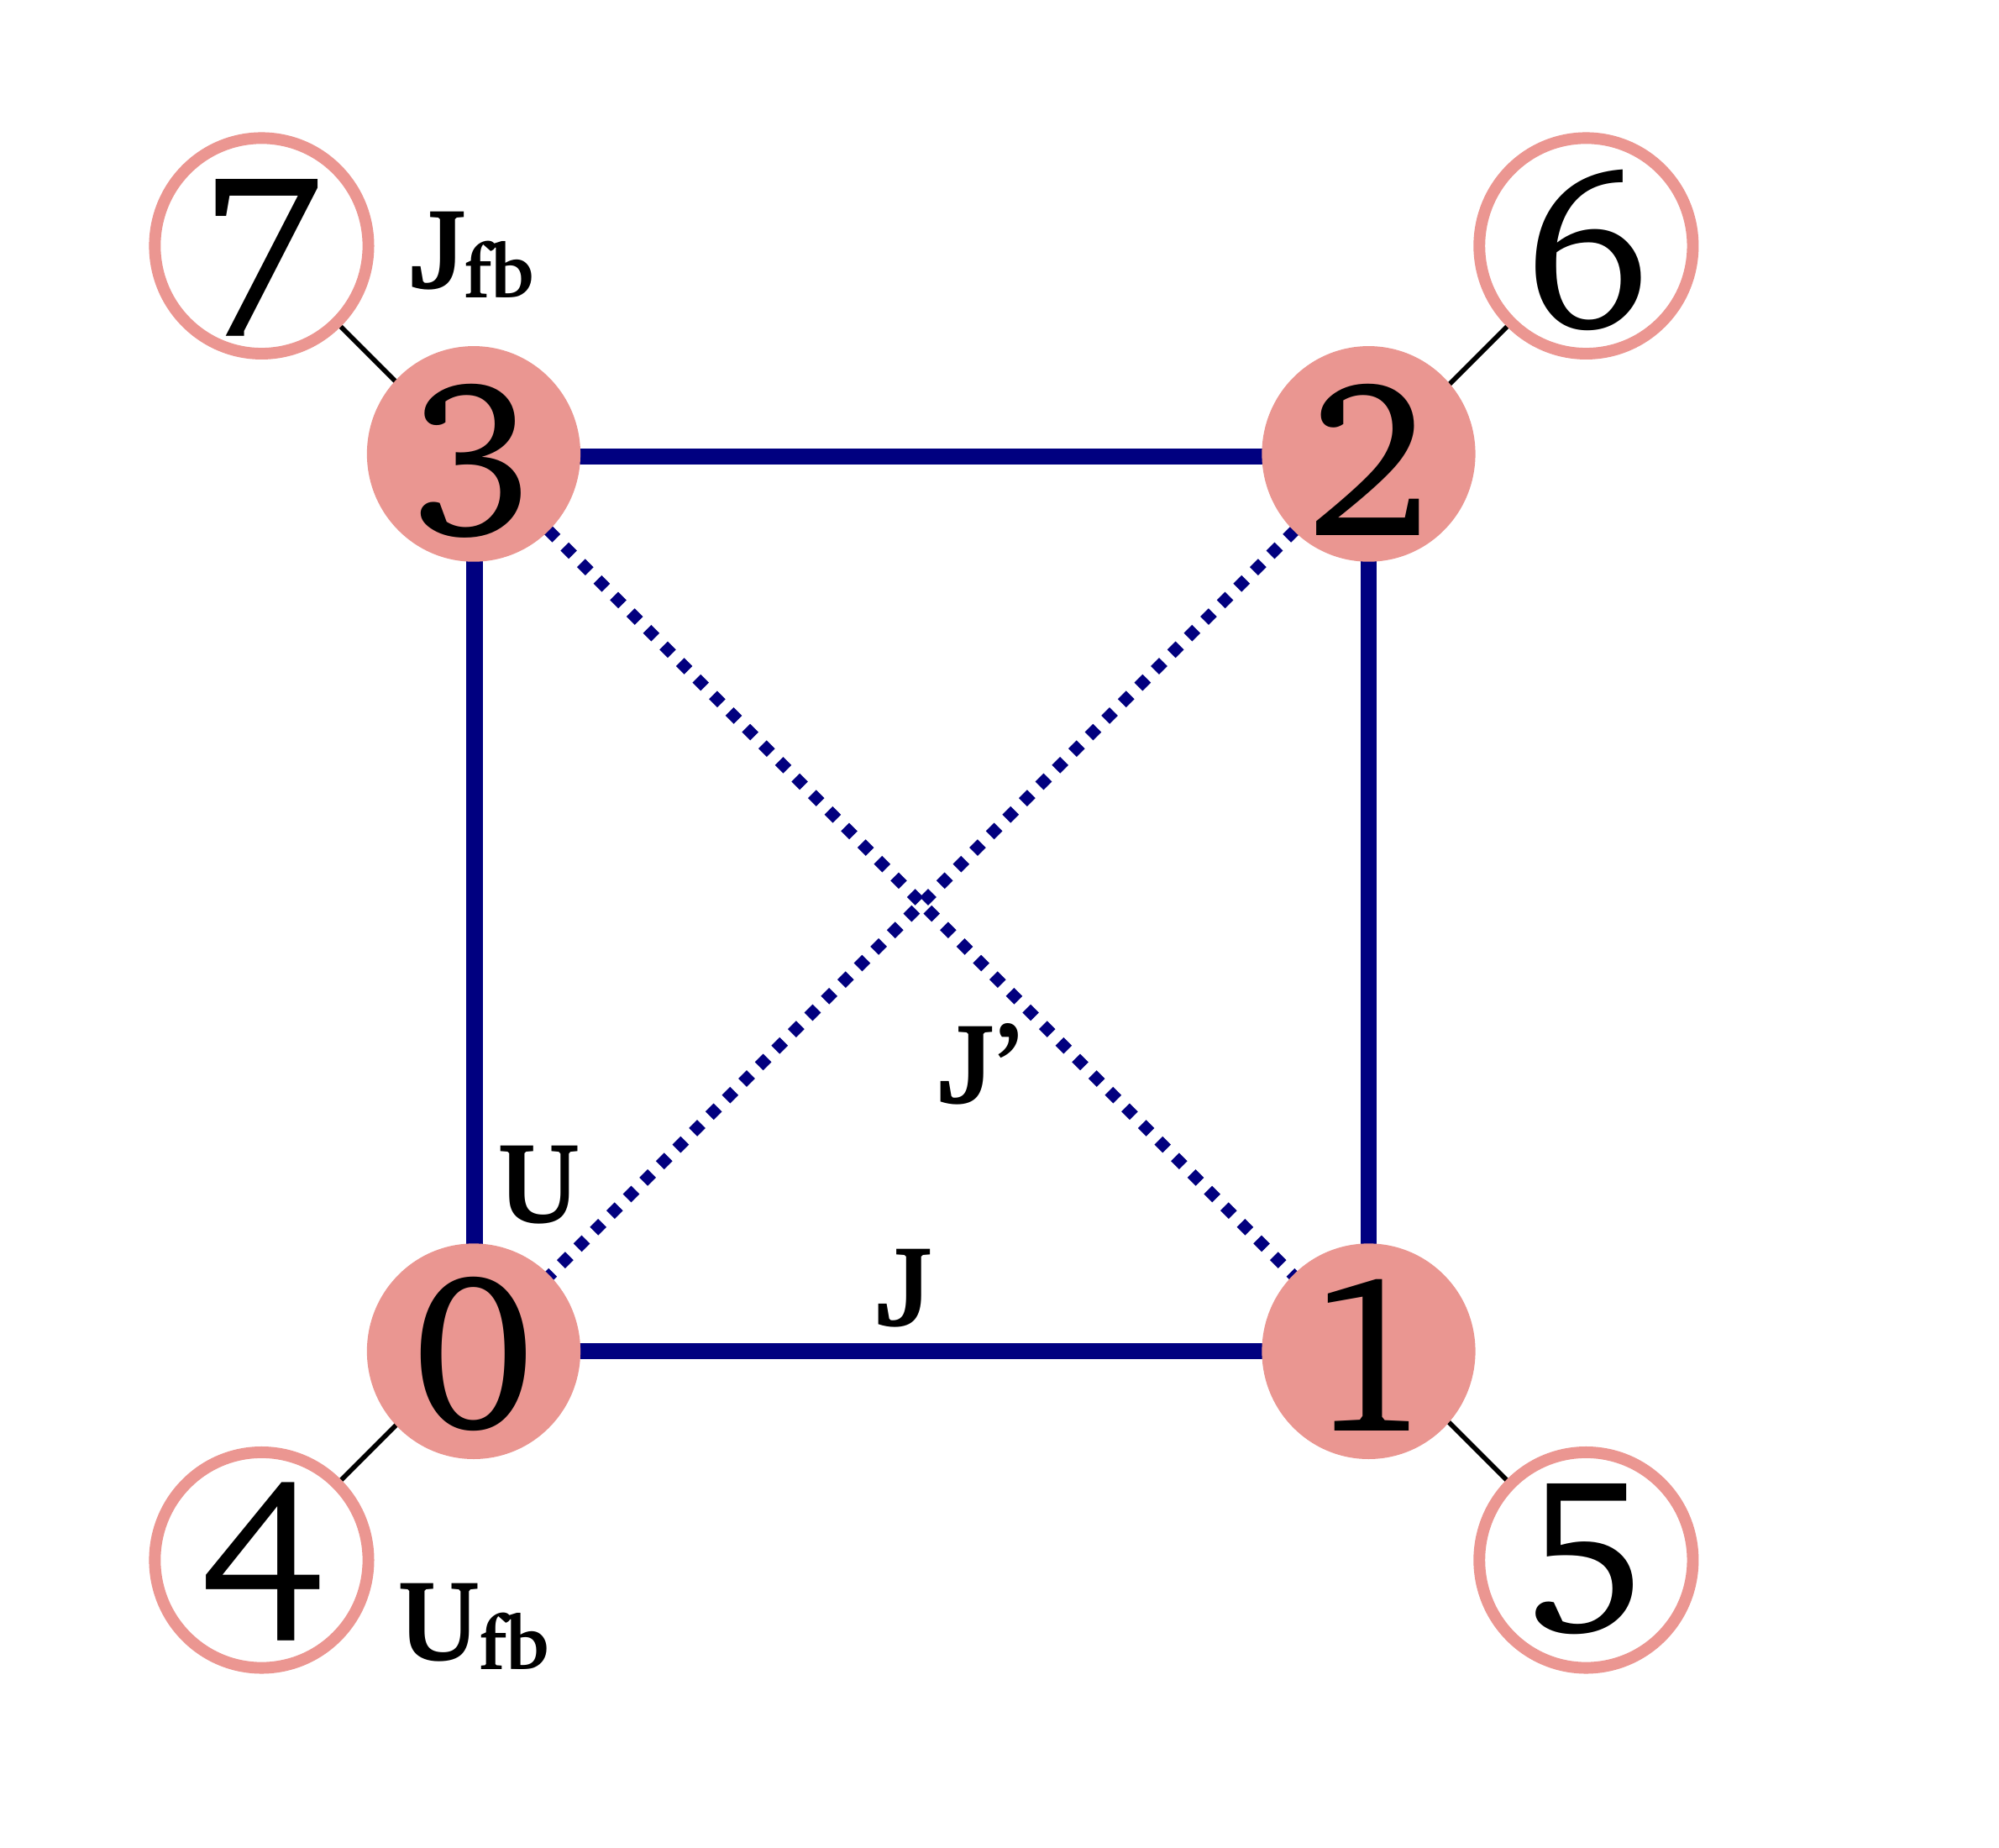
\includegraphics[width=0.92\linewidth,keepaspectratio]{fig_plaquette}\\[2pt]
            {\scriptsize Hubbard plaquette (atoms 0--3), one uncorrelated bath
                site each (4--7). $J_\text{fb}(t)$ smoothly switched on from
                $t=0$; $J$, $J'$ static.}

            \vspace{0.4em}
            {\scriptsize
                $U{=}5.56$,\ $J{=}2$,\ $J'{=}{-}0.6$,\ $J_\text{fb}{=}0.3$,\
                $\mu{=}0.479$,\ $\mu_\text{bath}{=}0.1$,\ $T{=}0.001$.}
        \end{column}
        \begin{column}{0.62\textwidth}
            \centering
            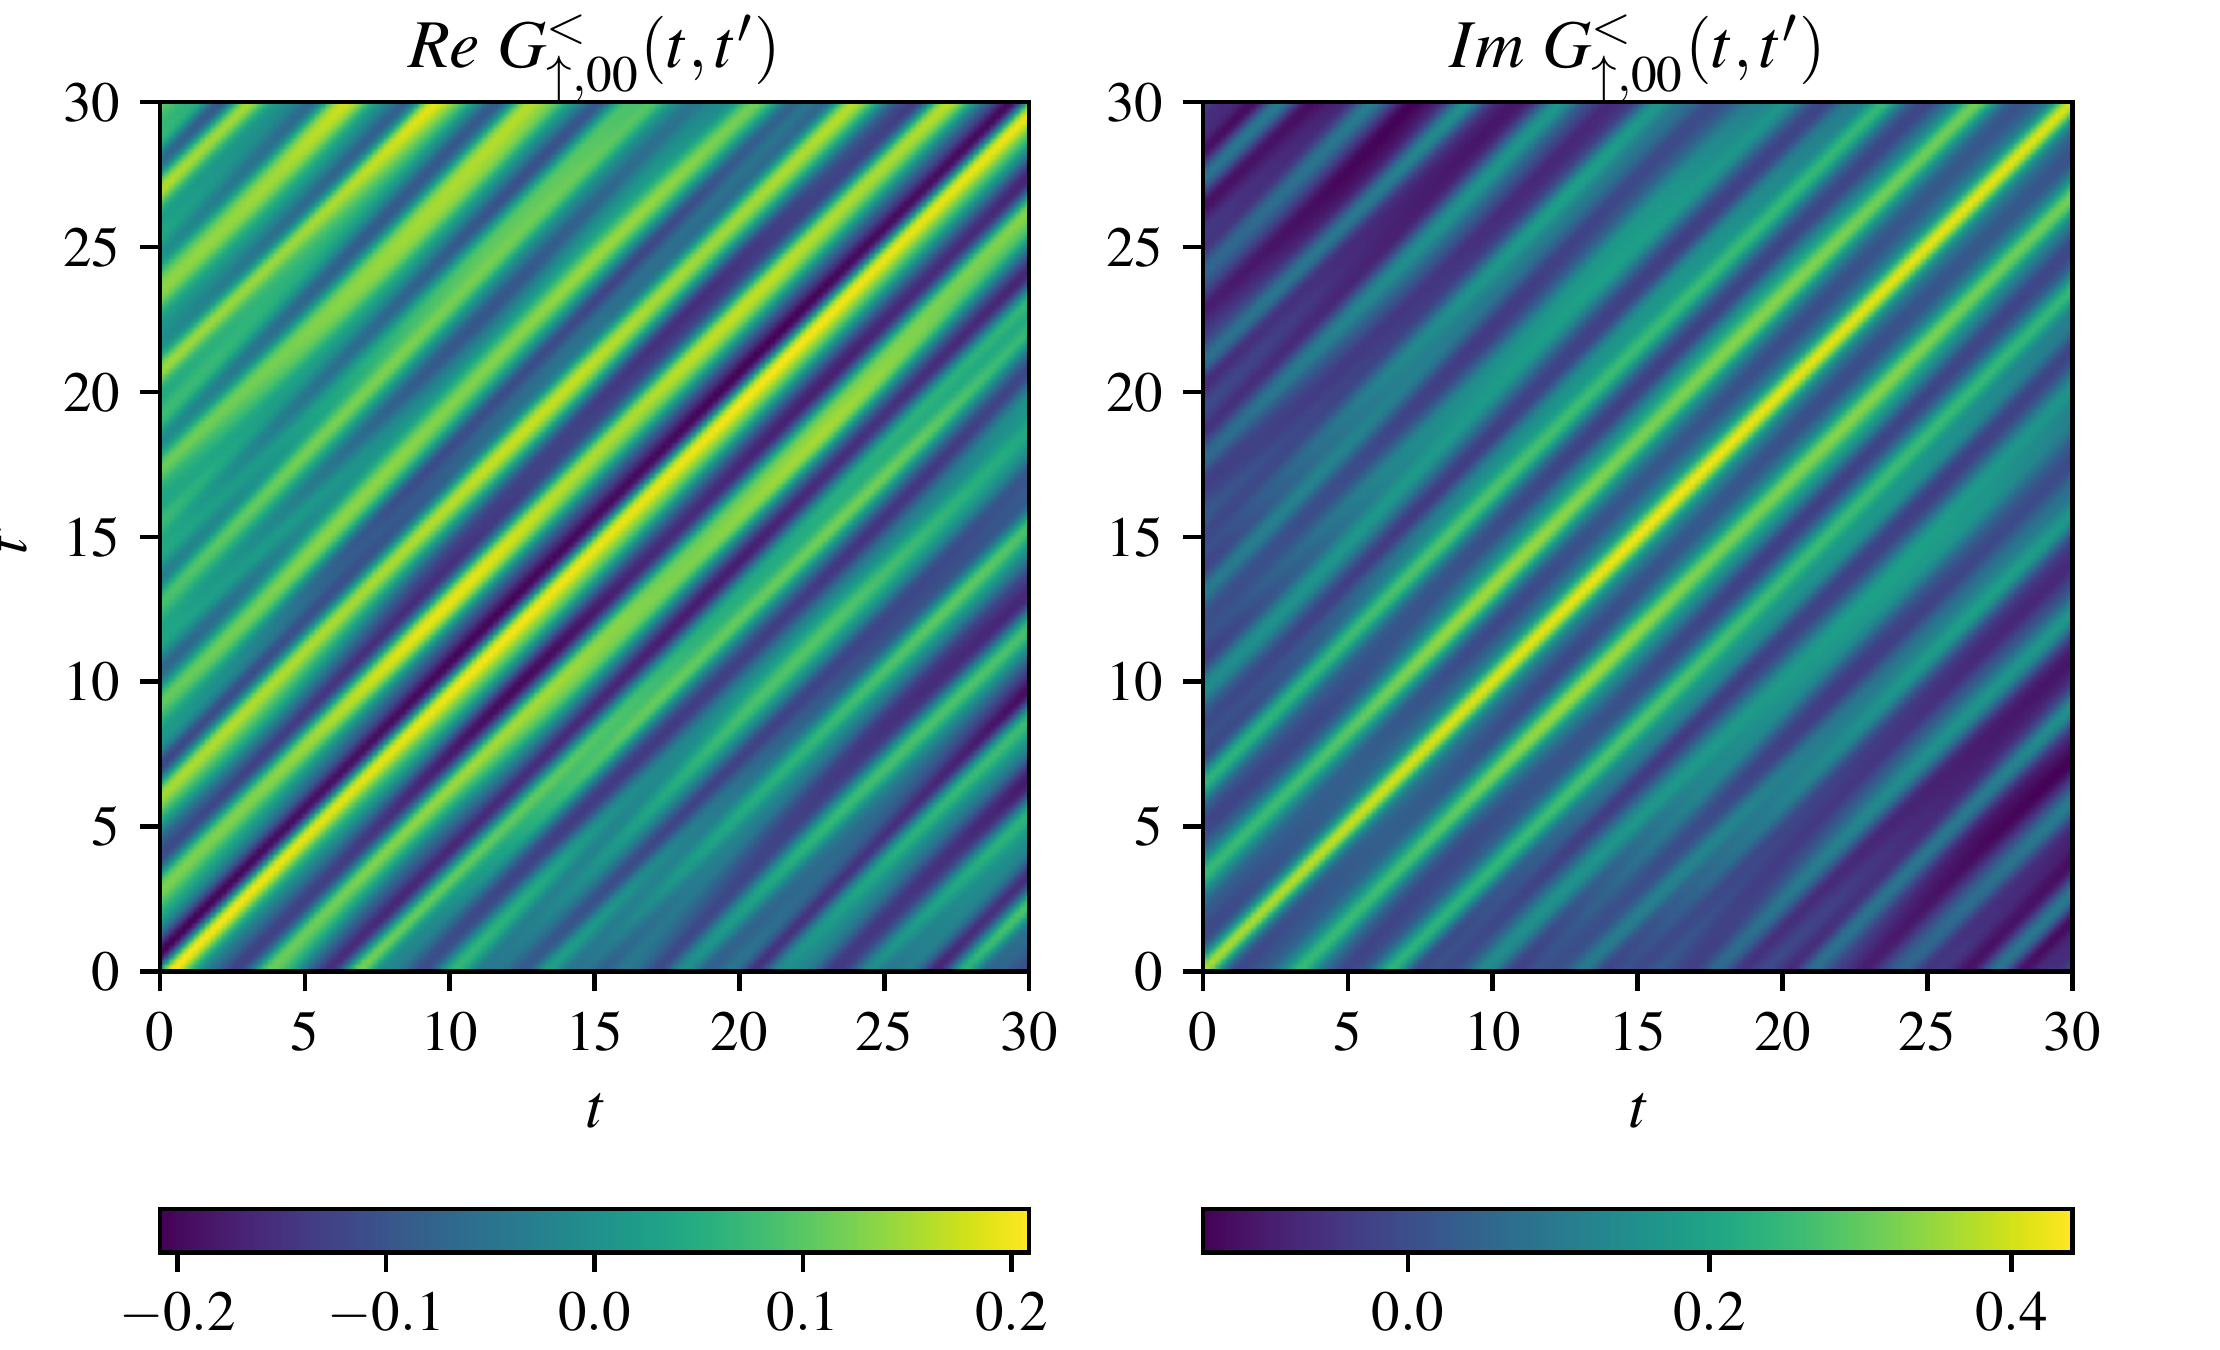
\includegraphics[width=\linewidth,keepaspectratio]{fig_g}\\[2pt]
            {\scriptsize Lesser Green's function $G^<_{\uparrow,00}(t,t')$ of
                impurity site $0$ after slow turn-on of $J_\text{fb}$.}
        \end{column}
    \end{columns}
    \hfill{\small Credits: V.~Valmispild}
    \vspace{0.3em}
\end{frame}

\begin{frame}{Results from \realevol\ — three-time correlator at fixed $t$}
    \centering
    {\small $\langle n_{\uparrow,0}(t)\,c^\dagger_{\downarrow,0}(t')\,
        c_{\downarrow,0}(t'')\rangle$ on the same plaquette + bath model;
        Re (left panel) / Im (right panel) of each pair.}

    \vspace{0.3em}
    \begin{columns}[T,onlytextwidth]
        \begin{column}{0.333\textwidth}
            \centering
            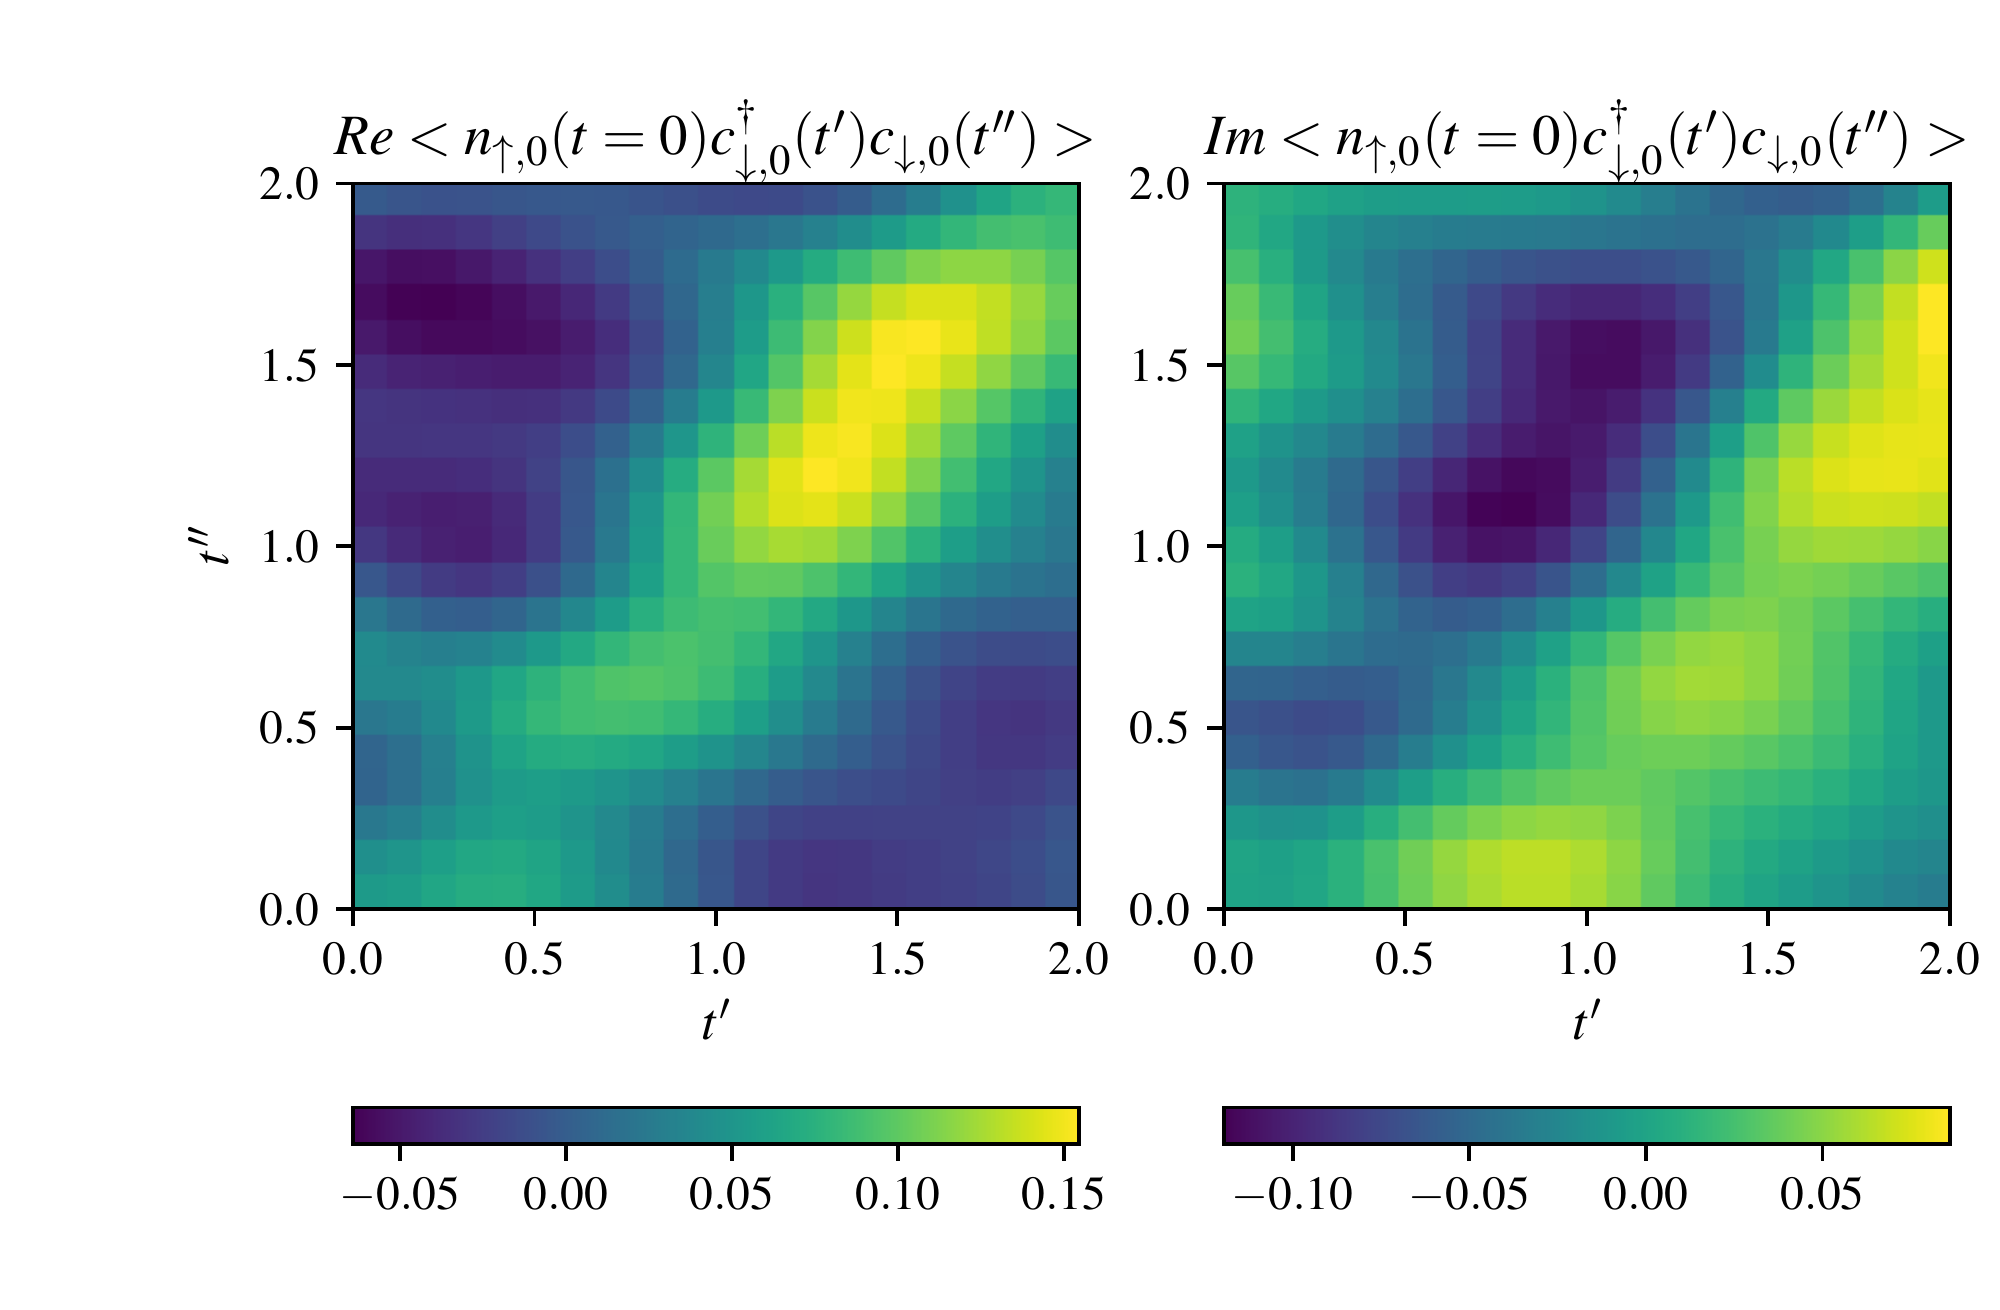
\includegraphics[width=\linewidth,keepaspectratio]{fig_3t_t0}\\[-2pt]
            {\footnotesize $t = 0$}
        \end{column}
        \begin{column}{0.333\textwidth}
            \centering
            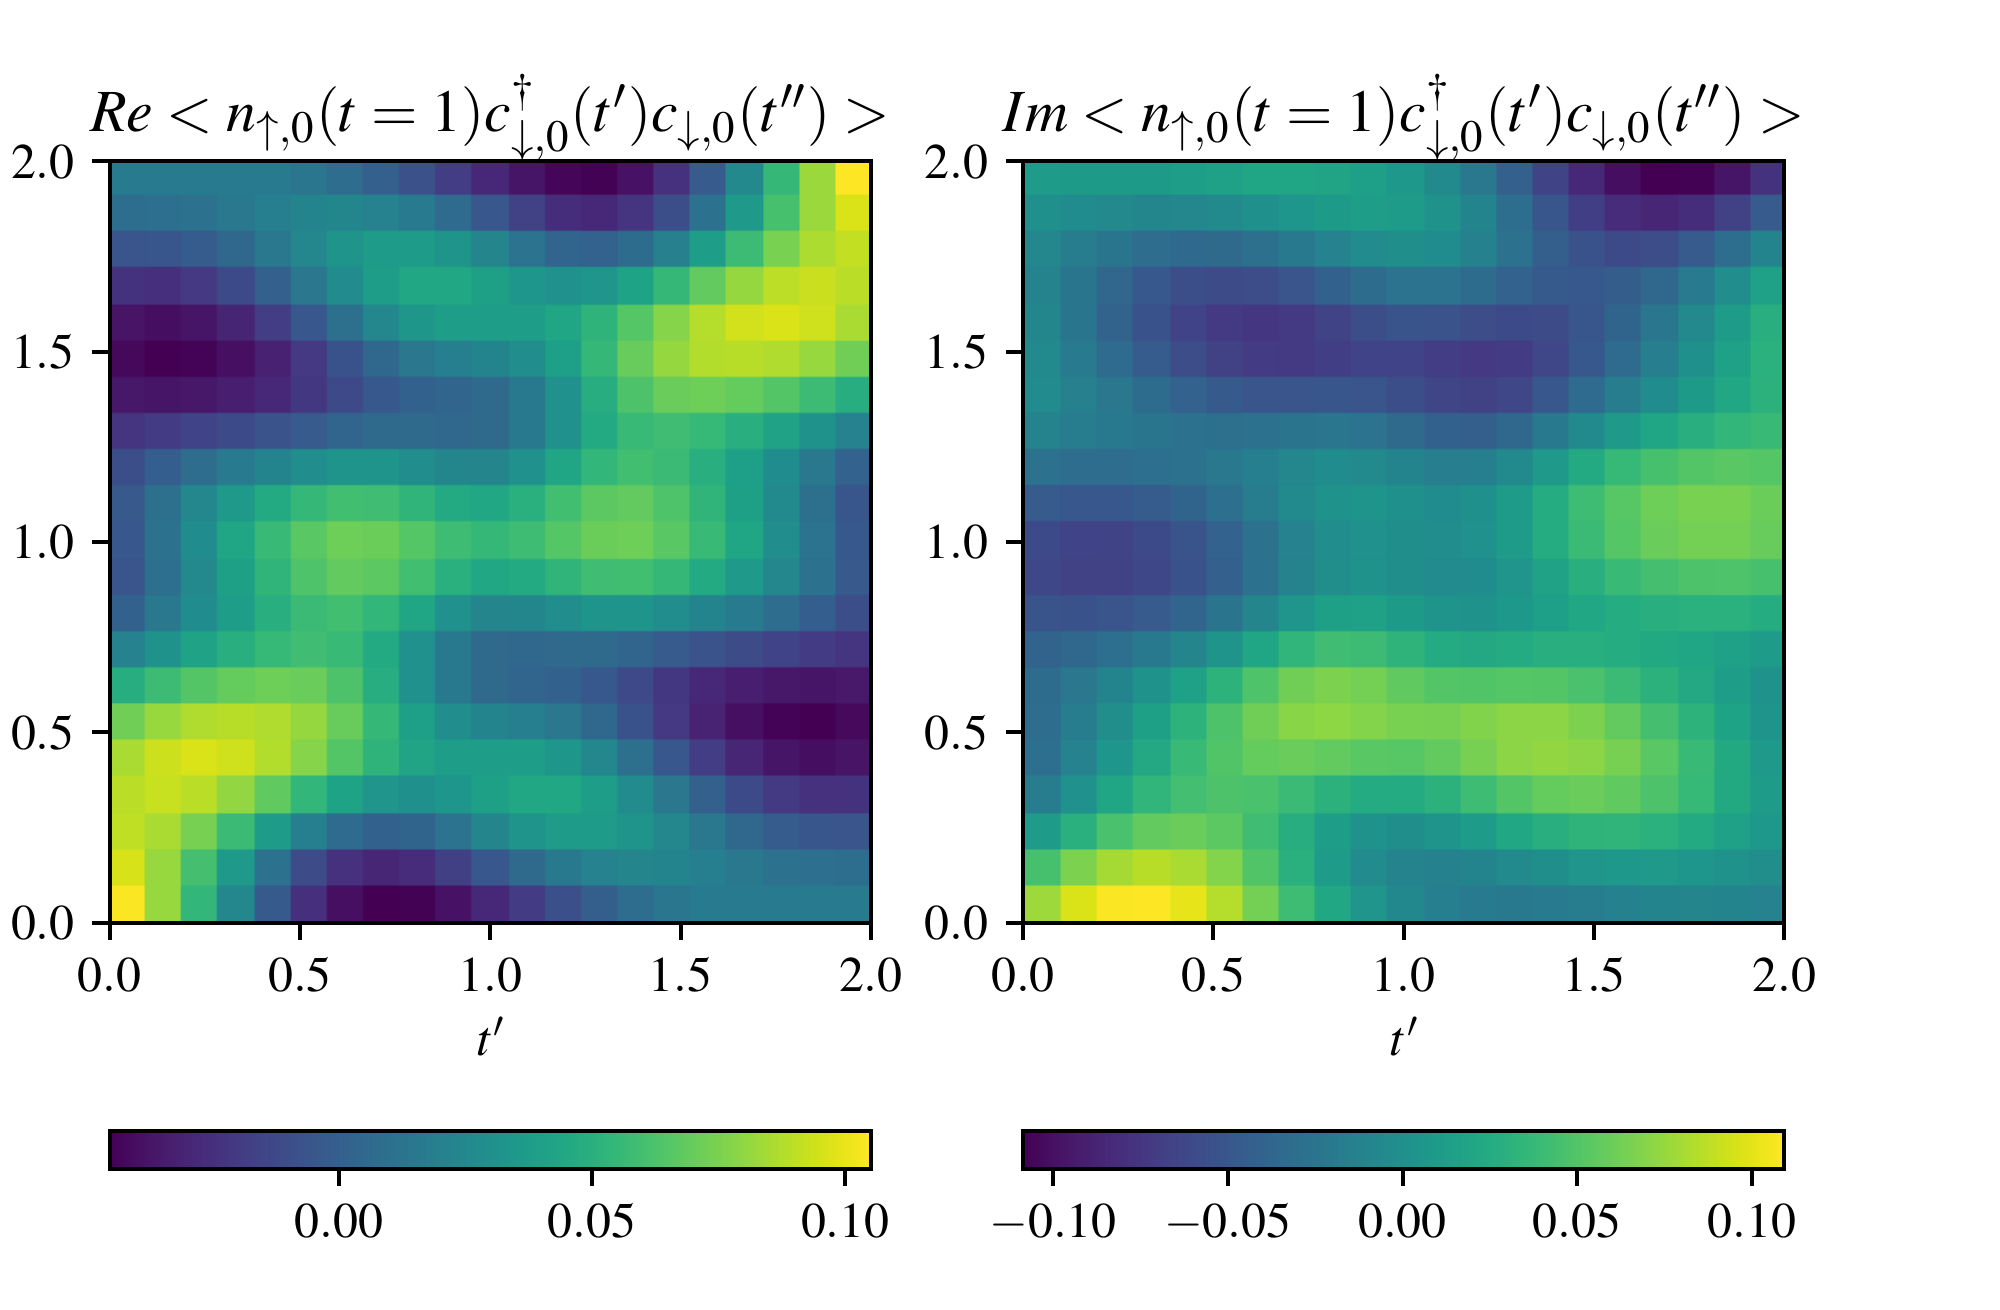
\includegraphics[width=\linewidth,keepaspectratio]{fig_3t_t1}\\[-2pt]
            {\footnotesize $t = 1$}
        \end{column}
        \begin{column}{0.333\textwidth}
            \centering
            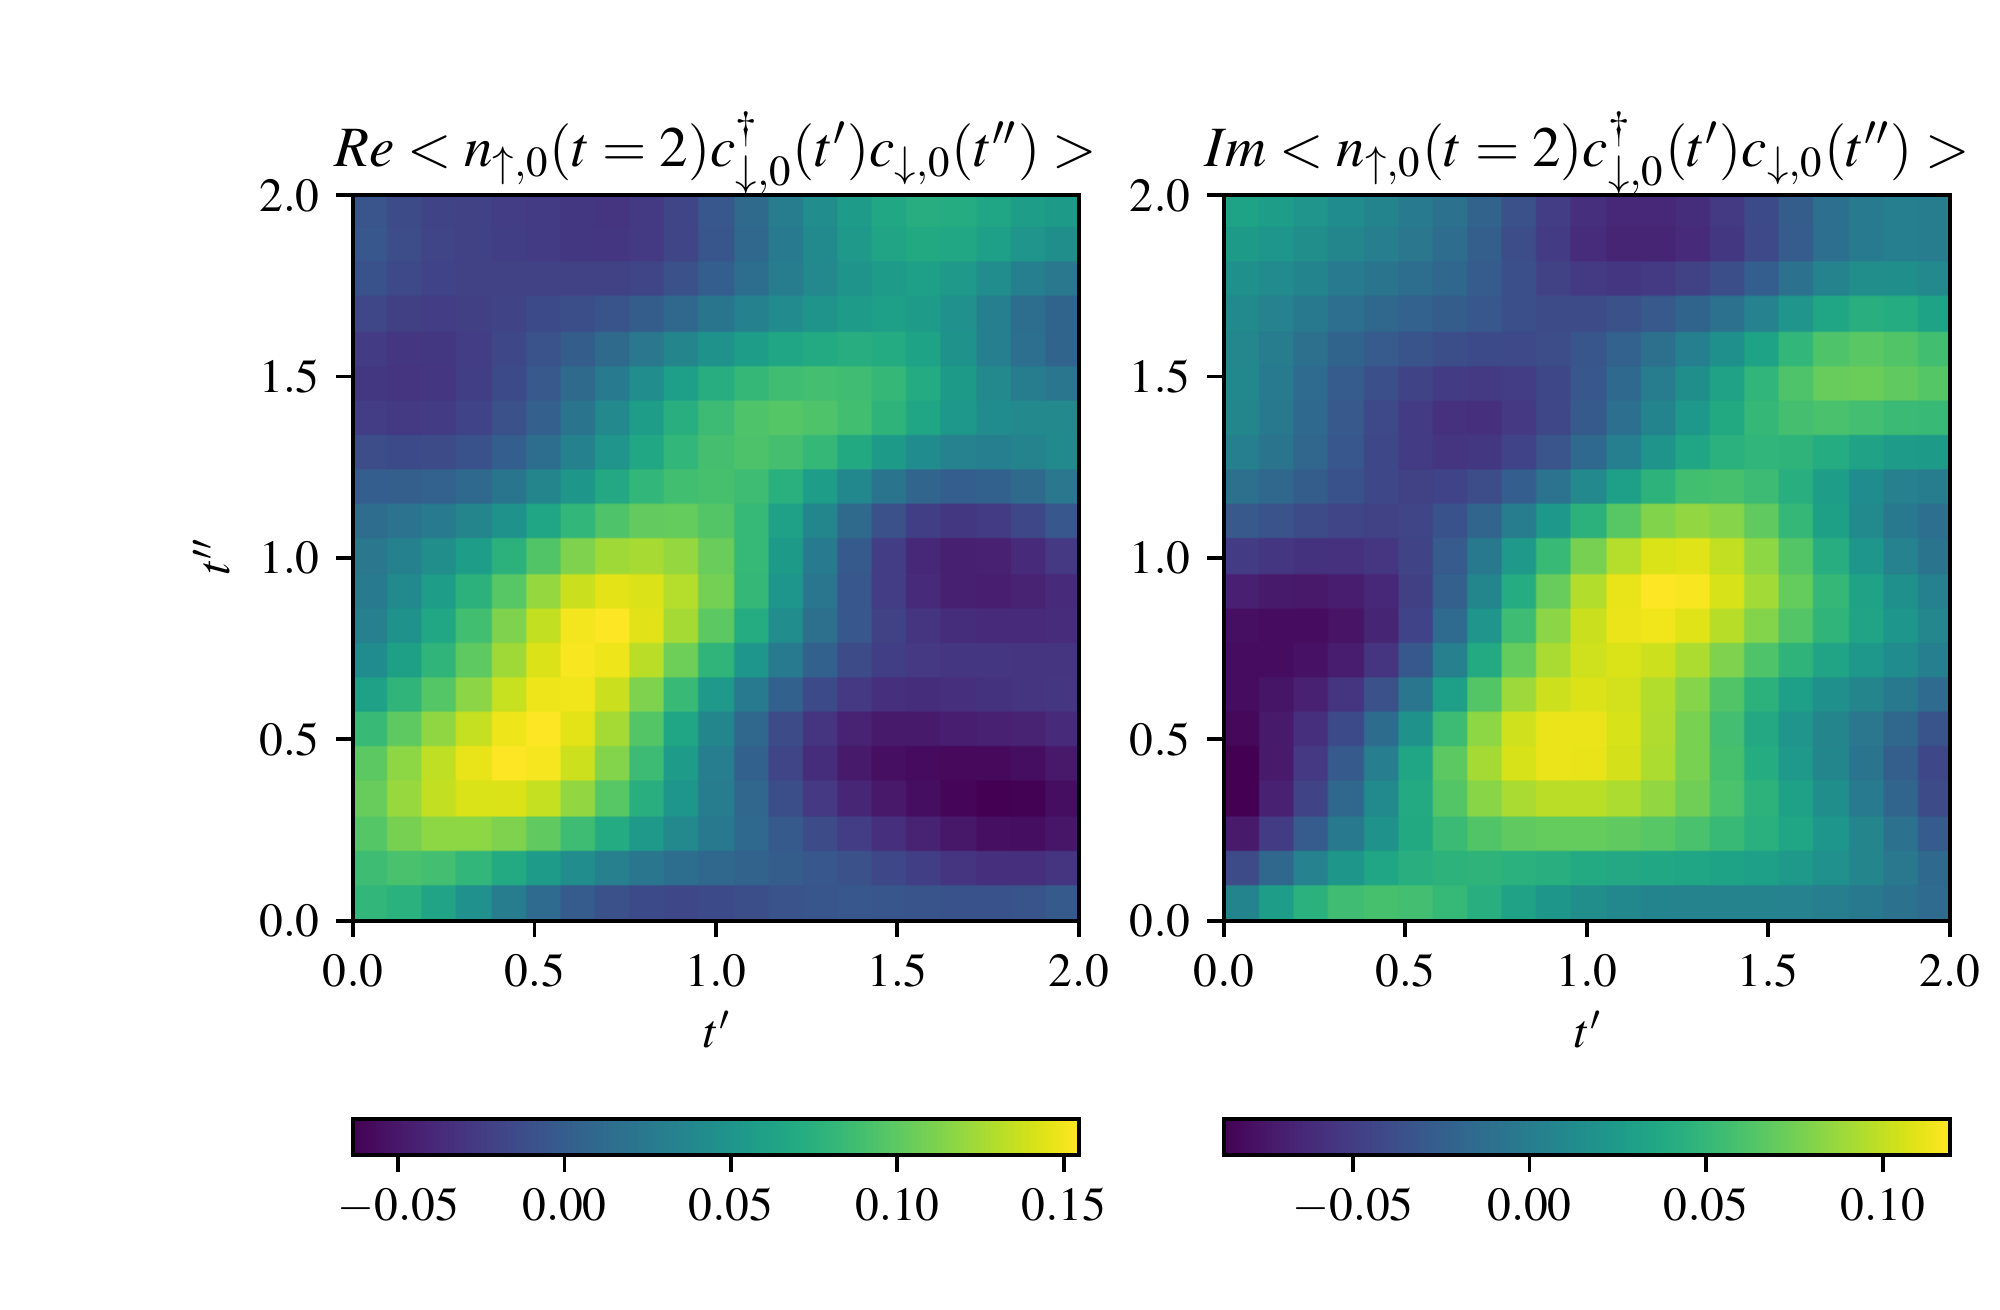
\includegraphics[width=\linewidth,keepaspectratio]{fig_3t_t2}\\[-2pt]
            {\footnotesize $t = 2$}
        \end{column}
    \end{columns}

    \vspace{0.4em}
    {\scriptsize Non-trivial $t$-dependence of the slices is exactly the
        retardation discarded by the instantaneous-vertex approximation.}

    \hfill{\small Credits: V.~Valmispild}
    \vspace{0.5em}
\end{frame}

% =========================================================================
\section{tddt — lattice solver}
% =========================================================================

\begin{frame}{\tddt\ — implementation of the lattice D-TRILEX equations}
    \begin{tikzpicture}[remember picture, overlay]
        \node[anchor=north east, xshift=-4pt, yshift=-4pt]
        at (current page.north east) {%
            \begin{tikzpicture}
                \node[fill=white, draw=black!20, inner sep=2pt, rounded corners=1pt]
                {\qrcode[height=1.6cm]{https://github.com/krivenko/tddt}};
        \end{tikzpicture}};
    \end{tikzpicture}
    \small
    \texttt{github.com/krivenko/tddt} (Python $\ge$ 3.10, \triqs\ 3.3.x).

    \medskip
    \begin{columns}[T,onlytextwidth]
        \begin{column}{0.5\textwidth}
            \textbf{What it does}
            \begin{itemize}
                \item Reads impurity input ($g$, $\chi$, $\Lambda$) from
                \realevol;
                \item builds non-local $\tilde G$, $W$ on the two-branch
                Keldysh contour with $\rho_0 = e^{-\beta H(0)}/Z$;
                \item assembles $\tilde\Sigmat$, $\tilde\Pi$ by doing four-time
                contour integrals for D-TRILEX diagrams;
                \item solves the Dyson equations for the dual fermionic and bosonic correlation functions;
                \item recovers lattice response functions of the real electrons from the dual correlators.
            \end{itemize}
        \end{column}
        \begin{column}{0.48\textwidth}
            \textbf{Design choices}
            \begin{itemize}
                \item pure Python for clarity and ease of use;
                \item \triqs-style containers for
                all contour Green's functions, susceptibilities and
                vertices;
                \item A multistep numerical integration scheme for contour convolutions (inspired by {\bf NESSi} package);
                \item heavy lifting via NumPy / SciPy, BLAS-backed
                tensor contractions;
                \item \texttt{pytest} test suite to ensure correctness;
                \item Extensive Jupyter tutorial: \texttt{doc/example.ipynb}.
            \end{itemize}
        \end{column}
    \end{columns}
\end{frame}

% =========================================================================
\section{Status \& outlook}
% =========================================================================

\begin{frame}{Status, bottlenecks and outlook}
    \textbf{Current status}
    \begin{itemize}
        \item \realevol\ v0.11.x: production-ready impurity solver, exact
        $\Lambda(t_1,t_2,t_3)$ measurement implemented and tested.
        \item \tddt: D-TRILEX diagrams and contour Dyson equations implemented and partially tested.
    \end{itemize}

    \medskip
    \textbf{Bottlenecks}
    \begin{itemize}
        \item Memory and CPU time for $\Lambda(t_1,t_2,t_3)$: $\mathcal{O}(N_t^3)$
        per spin/orbital block;
        \item lattice step: with sequential contraction (attach lines to
        one vertex at a time before contracting the two dressed
        vertices) the cost drops from $\mathcal{O}(N_t^6)$ to
        $\mathcal{O}(N_t^4)$ per $\bm k$ - i.e.\
        $\mathcal{O}(N_t^2)$ per external $(t,t')$ pair.
    \end{itemize}

    \medskip
    \textbf{Outlook}
    \begin{itemize}
        \item compressed representations of $\Lambda$ (tensor-train, orthogonal polynomials, IR);
        \item multi-orbital impurities (already supported by \realevol);
        \item application to driven Mott insulators \& spin dynamics.
    \end{itemize}
\end{frame}

% --- 21. Summary ---------------------------------------------------------
\begin{frame}{Summary}
    \begin{itemize}
        \item We are implementing the \textbf{full} time-dependent D-TRILEX
        scheme on the two-branch Keldysh contour - keeping the
        three-point vertex as a true three-time object.
        \item Two open-source codes carry the implementation:
        \begin{itemize}
            \item \realevol\ (\triqs/C++/Python): exact real-time impurity solver,
            including measurement of $\Lambda(t_1,t_2,t_3)$;
            \item \tddt\ (\triqs/Python): lattice solver assembling
            $\tilde\Sigma$, $\tilde\Pi$ from the four-time formulas
            and running the self-consistency loop.
        \end{itemize}
        \item Backbone of the real-time impurity part: a short-time,
        Krylov-based propagation scheme for finite quantum systems
        with explicit $\hat H(t)$ (Balzer et al, J. Phys.: Condens. Matter 24 035603 (2011)).
        \item First production applications and benchmarks against the
        recent \dgw\ method are in progress.
    \end{itemize}

    \vspace{1em}
    \begin{center}\small
        \texttt{github.com/krivenko/triqs-realevol}\\
        \texttt{github.com/krivenko/tddt}\\[2pt]
        \emph{Funded by ERC Grant 854843-FASTCORR}
    \end{center}
\end{frame}

\end{document}
